\section{Desarrollo}


\subsection{\textit{Data augmentation}}
Para la práctica se cuenta con un conjunto de datos basados en imágenes de distintos objetos en distintos espacios, a fin de que la red diseñada sea capaz de reconocer y localizar objetos de cuatro clases: `botella', `silla', `mesa' y `sofá'.

A fin de poder mejorar el entrenamiento de la red, se han llevado a cabo una serie de transformaciones sobre el conjunto de imágenes originales para así proveer al conjunto de entrenamiento de una mayor variación y un mayor número de datos de entrenamiento\footnote{El código de estas transformaciones se encuentra en \texttt{src/data\textunderscore augmentation.py}.}. Todas las transformaciones son aleatorias, ya que al ejecutar cada \textit{epoch} se generará una nueva versión.

Dado que el \textit{dataset} trabaja con imágenes con la librería Pillow\footurl{https://python-pillow.org}, decidimos usar las transformaciones de la librería torchvision\footurl{https://pytorch.org/vision}, ya que permiten trabajar con este formato. La clase \texttt{torchvision.transforms.ColorJitter\footurl{https://pytorch.org/vision/stable/generated/torchvision.transforms.ColorJitter}} permite modificar los parámetros cromáticos de una imagen dada, como el brillo, contraste, saturación y matiz. En la implementación actual, tras experimentar con diferentes valores, se usan valores de 0.28 para el brillo, 0.3 para contraste y saturación, y 0.06 para el matiz, que aunque pueda resultar bajo, permite mantener los colores en términos generales entre tonos marrones o amarillos/rojos oscuros (colores que pueden ser alterados por la luz natural o bombillas), ya que a valores más elevados comienzan a aparecer colores que no serían naturales.

Se decidió no incluir otras transformaciones de rotación o recorte de las imágenes, ya parte de los objetos podría quedar fuera del campo visible, lo cual provocaba peores resultados en el modelo.

En la Figura \ref{fig:data_aug} se pueden observar ejemplos de posibles transformaciones de la imagen original (\ref{fig:sample_og}).


\begin{figure}[h]
  \centering
  \begin{subfigure}{.3\textwidth}
    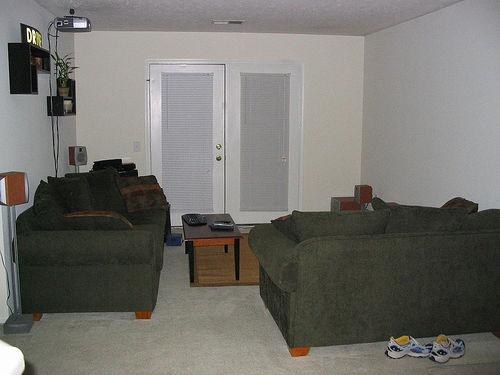
\includegraphics[width=\linewidth]{sample_og.jpg}
    \caption{Imagen original}
    \label{fig:sample_og}
  \end{subfigure}
  \multido{\i=1+1}{5} {
    \begin{subfigure}{.3\textwidth}
      \includegraphics[width=\linewidth]{sample_v\i.jpg}
      \caption{Transformación \i}
      \label{fig:sample_\i}
    \end{subfigure}
    \ifthenelse{\equal{\i}{2}}
      {\\\medskip}  % new row
      {}
  }
  \caption{Ejemplo de transformaciones aplicadas a una imagen}
  \label{fig:data_aug}
\end{figure}


\subsection{Influencia de los Umbrales en la Inferencia}
Viendo la Figura \ref{fig:objectness_TH_SCORE} del Objectness-RPN, a medida que se aumenta el TH\textunderscore SCORE aumenta la precisión y disminuye el \textit{recall}, esto se debe a que el modelo es más selectivo en la detección de regiones. Mientras que en la Figura \ref{fig:global_TH_SCORE}, podemos ver que se mantiene estable, por lo tanto el clasificador no se ve afectado.

\begin{figure}[h]
  \centering
  \begin{subfigure}[t]{.5\textwidth}
    \includesvg[width=\linewidth]{Objectness-RPN_th_score}
    \caption{Objectness-RPN}
    \label{fig:objectness_TH_SCORE}
  \end{subfigure}%
  \begin{subfigure}[t]{.5\textwidth}
    \includesvg[width=\linewidth]{Global-Classification_th_score}
    \caption{Global Classification}
    \label{fig:global_TH_SCORE}
  \end{subfigure}
  \caption{TH\textunderscore SCORE}
\end{figure}

Como se puede observar en la Figura \ref{fig:objectness_TH_IOU}, a medida que se aumenta el umbral para determinar si una región se considera correcta o no, se reducen todas las métricas, esto se debe a que es difícil para nuestro modelo detectar las regiones correctas. Mientras que para el clasificador en la Figura \ref{fig:global_TH_IOU} podemos ver que se mantiene estable, por lo tanto el clasificador no se ve afectado.

\begin{figure}[h]
  \centering
  \begin{subfigure}[t]{.5\textwidth}
    \includesvg[width=\linewidth]{Objectness-RPN_th_iou}
    \caption{Objectness-RPN}
    \label{fig:objectness_TH_IOU}
  \end{subfigure}%
  \begin{subfigure}[t]{.5\textwidth}
    \centering
    \includesvg[width=\linewidth]{Global-Classification_th_iou}
    \caption{Global Classification}
    \label{fig:global_TH_IOU}
  \end{subfigure}
  \caption{TH\textunderscore IOU}
\end{figure}



\subsection{\textit{Anchors}}
    Analizando las salidas del modelo, y comparando los \textit{anchors} empleados
    (su tamaño y relación de aspecto) con las \textit{bounding boxes} de las imágenes proporcionadas,
    se puede observar que la distribución de las predicciones, con respecto a la relación de aspecto
    y el tamaño es bastante similar a la verdad objetiva (Figura \ref{fig:ratio_v_box}).

    \rasterfigure[0.9]{ratio_v_box}{Relación entre la relación de aspecto y las bounding boxes}

    Debido a los \textit{anchors} empleados, los objetos que mejor se detectan suelen ser
    los que tienen \textit{bounding boxes} con una relación de aspecto más cercana a uno (Figura \ref{fig:ratio_v_anchors}).
    Por lo que las sillas, que tienen \textit{bounding boxes} más `cuadradas', se predicen mejor con este modelo.

    \rasterfigure[0.9]{ratio_v_anchors}{Relación entre la relación de aspecto y los anchors}

    En cuanto al tamaño de los \textit{anchors}, se predicen mejor los objetos más grandes,
    seguramente a que la reducción del tamaño de la imagen hace que se pierda algo de información.

    Como conclusión de esta sección, se podría mejorar el modelo añadiendo
    \textit{anchors} con una relación de aspecto algo superior (3:1, o 4:1) para captar
    los objetos en esa sección que no se están percibiendo. De igual manera,
    se podría probar a añadir \textit{anchors} de menor tamaño, para captar las botellas o de
    mayor tamaño, para captar mejor las mesas o los sofás.



\subsection {\textit{RoI pooling} y clasificación}
    La técnica de \textit{RoI pooling} resulta de gran eficacia a la hora de clasificar y detectar objetos pues busca normalizar el tamaño de las regiones en las que pondrá atención el modelo para que sean uniformes y evitar que la diferencia de tamaño pueda distorsionar los resultados. Es posible extraer la clase de un objeto a partir de la RoI si se trata de objetos que no sean muy similares en cuanto a forma, ya que será posible detectar variaciones en la activación del mapa, pero si se trata de objetos similares en forma aumenta el riesgo de confusión.

    Por ejemplo, en el caso de una objeto `botella' y otro `silla', será factible clasificarlos teniendo únicamente en cuenta la RoI, ya que en el caso de la botella la actividad se concentrará en forma vertical en el centro de la región, mientras que la silla mostrará mayor activación en las zonas cercanas a los bordes donde generalmente se encontrarán las patas y respaldo.

    La matriz de confusión generada (Figura \ref{fig:dconf}) resulta de gran utilidad para comprobar si realmente el modelo está siendo de capaz de clasificar correctamente los objetos de cada clase y poder comprobar cuáles son aquellos que se confunden entre sí con mayor frecuencia.

    \rasterfigure{dconf}{Matriz de confusión}

    Para interpretar la matriz de confusión se tiene en cuenta que la diagonal principal representa los aciertos, es decir, los objetos que se han clasificado correctamente como su clase. En ella primeramente se observa que la clase botella no se ha confundido con las otras clases, mientras que entre las otras tres clases sí que ha habido cierto grado de confusión entre ellas, especialmente entre `sofá' y `silla'.

    Esto se debe a que tanto `sofá' como `mesa' y `silla' comparten múltiples características al ser todos muebles, tener varias patas sobre las que apoyarse, superficie plana, tamaños similares y poder encontrarse en entornos similares como puede ser un comedor. Por otro lado, la clase `botella' apenas comparte características con ellas al tratarse de objetos mayormente de otro material, plástico, tamaño por lo general bastante menor y carecer de elementos característicos comunes a las otras clases como las patas.

    A fin de mejorar la clasificación, podría ser interesante, ya que se conocen que clases se confunden más, incluir más imágenes de entrenamiento que incluyan objetos de clase `sofá' y `silla' desde más ángulos o en mayor variedad de entornos.



